\documentclass[aspectratio=169]{beamer}


\usepackage[utf8]{inputenc}
\usepackage{amsmath}
\usepackage{amsfonts}
\usepackage{amssymb}
\usepackage{graphicx}
\usepackage{ragged2e}  % `\justifying` text
\usepackage{booktabs}  % Tables
\usepackage{tabularx}
\usepackage{tikz}      % Diagrams
\usetikzlibrary{calc, shapes, backgrounds}
\usepackage{amsmath}
\usepackage{amssymb}
\usepackage{dsfont}
\usepackage{url}       % `\url
\usepackage{listings}  % Code listings
\usepackage[T1]{fontenc}
%%%%
\usepackage[style=authortitle,backend=bibtex]{biblatex}
\addbibresource{bibliography.bib}
%%%%

\usepackage{theme/beamerthemehbrs}

\author[Jain]{Gautam Kumar Jain}
\title{End-to-End Prediction of Driving
Commands Using 3D Lane Detection as an
Auxiliary Task}
%\subtitle{Subtitle of presentation}
\institute[HBRS]{Hochschule Bonn-Rhein-Sieg}
\date{\today}
\subject{Test beamer}

% leave the value of this argument empty if the advisors
% should not be included on the title slide
\def\advisors{Prof. Dr Paul G. Plöger , Prof. Dr. Sebastian Houben, Prof. Dr. Arun K. Singh}

%\thirdpartylogo{images/uni_tartu_logo.png}


\begin{document}
{
\begin{frame}
\titlepage
\end{frame}
}

%%%% _________ Introduction________%%%%%
\begin{frame}{Problem Statement}
    \begin{itemize}
        \item This project aims at predicting driving commands and 3D road lanes using a sequence of monocular images.
        \item The whole scenario can be seen as a multi-task learning problem.
        \item Prediction of driving commands is considered as main task and the prediction of 3D lanes is the auxiliary task.
        \item The project further aims to investigate the following: 
        \begin{itemize}
            \item Can 3D lane detection improve the prediction of driving commands? 
            \item Is the whole pipeline more interpretable by the introduction of auxiliary task.
            \item Can multitask learning improve generalizaton? 
            \item Can task loss balancing favor the performance of the main task? 
        \end{itemize}
    \end{itemize}
\end{frame}
%---Motivation---%
\begin{frame}{Motivation (1/6)}
  \textbf{A Driving scenario in autonomous driving}
  place a picture of the road scenario
\end{frame}

%%%%  next frame %%%
\begin{frame}{Motivation (2/6)}
  \textbf{End-to-End Autonomous Driving}
  \begin{itemize}
    \item Research done in autonomous driving is focused on two approaches \footcite{DBLP:journals/corr/abs-2003-06404}
        \begin{itemize}
            \item Modular 
            \item End-to-end 
        \end{itemize}
        
  \end{itemize}
    \begin{figure}[H]
     \centering
     
\begin{subfigure}{\textwidth}
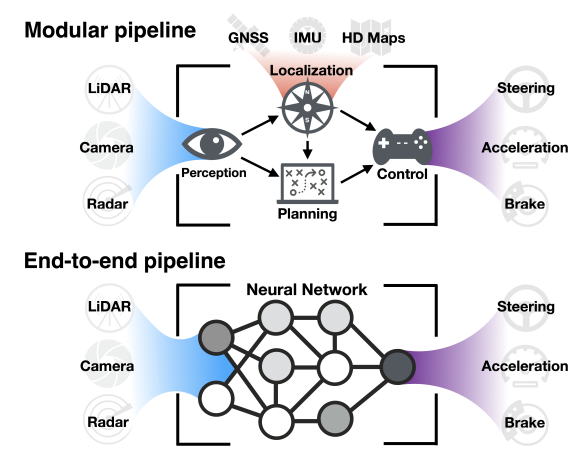
\includegraphics[width=0.4\linewidth, height=3.2cm]{images/end-modular.png} 
\label{fig:subim1}
\end{subfigure}

\caption{Modular and end-end pipelines for autonomous driving\footcite{DBLP:journals/corr/abs-2003-06404}}
\label{fig:image2}
\end{figure}
\end{frame}

%--- Next Frame ---%
\begin{frame}{Motivation (2/6)}
  \textbf{Multi task Learning vs Auxiliary Learning}

  \begin{itemize}
      \item By definition, both multi-task learning and auxiliary learning is the same. 
      \item In both cases we learn for multiple tasks by the sharing the same feature representation
  \end{itemize}
\end{frame}

%--- Next Frame ---%
\begin{frame}{Motivation (3/6)}
  \textbf{Challenges in end-to-end autonomous driving}

  \begin{itemize}
      \item Causal confusion
      \item Distribution shift 
      \item Selection of auxiliary tasks
  \end{itemize}
\end{frame}



\begin{frame}
\printbibliography
\end{frame}
\end{document}
